\section{An interconnection perspective}
\label{sec:io_stable}

The reason of exploring the consistency between two approaches is that I try to find a pattern that can be applied to a class of multi-agent system ``consensus-seeking'' problems.
The system can be modeled as a structure in Figure \ref{fig:consensus_seeking}.
The consistency in two algorithms proposed in Dr. Ren's paper \cite{5229134} shows that the control law can be decomposed into two parts.
One part is applied for consensus seeking to generate $ \sigma^{d}_{i} $, the other part is applied to drive $ \sigma_{i} $ approaching to $ \sigma^{d}_{i} $.
This idea is inspired by another paper \cite{1470210}, which has a consensus scheme and a coordinate scheme.
A hypothesis is proposed but still needed a theoretical analysis and proof.
\begin{hyp}
\label{hyp:one}
A multi-agent system converges to a reference if there are 
\begin{itemize}
\item a parallel interconnection of all the agents and any agent $ i $'s $ \sigma_{i} $ converges to an input reference $ \sigma^{d}_{i} $ ;
\item a consensus seeking component guarantees that $ \forall i \forall j, \sigma_{i} \rightarrow \sigma_{j} $ as $ t \rightarrow \infty $;
\item a feedback interconnection of two component makes the system stable.
\end{itemize}
\end{hyp}


\begin{figure}
\centering
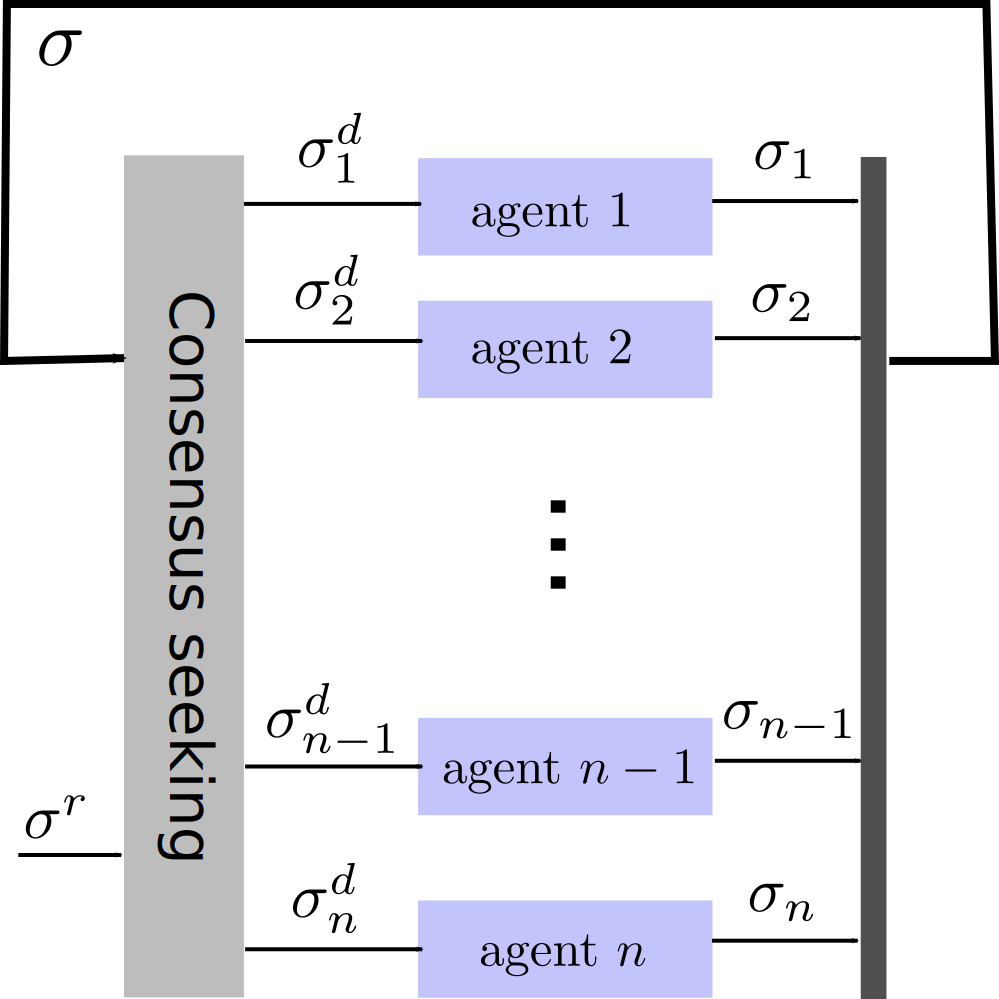
\includegraphics[width=0.4\linewidth]{./images/consensus_seeking}
\caption{Inter-connection representation of the multi-agent system.}
\label{fig:consensus_seeking}
\end{figure}